\chapter{Linear Methods for Regression}

\begin{exer}
  Show that the $F$ statistic for dropping a single coefficient from a model is equal to the square of the corresponding $z$-score.
\end{exer}

\begin{proof}
  Recall that the $F$ statistic is defined by the following expression \[
    \frac{(RSS_0 - RSS_1) / (p_1 - p_0)}{RSS_1 / (N - p_1 - 1)}.
  \] where $RSS_0, RSS_1$ and $p_0 + 1, p_1 + 1$ refer to the residual sum of squares and the number of free parameters in the smaller and bigger models, respectively.  Recall also that the $F$ statistic has a $F_{p_1 - p_0, N-p_1 - 1}$ distribution under the null hypothesis that the smaller model is correct.

  Next, recall that the $z$-score of a coefficient is \[
    z_j = \frac{\hat \beta_j}{\hat \sigma \sqrt{v_j}}
  \] and under the null hypothesis that $\beta_j$ is zero, $z_j$ is distributed according to a $t$-distribution with $N-p-1$ degrees of freedom. 

  Hence, by dropping a single coefficient from a model, our $F$ statistic has a $F_{1, N-p - 1}$ where $p + 1$ are the number of parameters in the original model.  Similarly, the corresponding $z$-score is distributed according to a $t_{N-p-1}$ distribution, and thus the square of the $z$-score is distributed according to an $F_{1, N-p-1}$ distribution, as required.

  Thus both the $z$-score and the $F$ statistic test identical hypotheses under identical distributions.  Thus they must have the same value in this case.    
\end{proof}

\begin{exer}
    Given data on two variables $X$ and $Y$, consider fitting a cubic polynomial regression model $f(X) = \sum_{j=0}^{3} \beta_j X^j$.  In addition to plotting the fitted curve, you would like a 95\% confidence band about the curve.  Consider the following two approaches:

\begin{enumerate}
    \item At each point $x_0$, form a 95\% confidence interval for the linear function $a^T \beta = \sum_{j=0}^{3}\beta_j x_0^j$.  
    \item Form a 95\% confidence set for $\beta$ as in (3.15), which in tun generates confidence intervals for $f(x_0)$.  
\end{enumerate}

   How do these approaches differ?  Which band is likely to be wider?  Conduct a small simulation experiment to compare the two methods.
\end{exer}

\begin{proof}
    The key distinction is that in the first case, we form the set of points such that we are 95\% confident that $\hat f(x_0)$ is within this set, whereas in the second method, we are 95\% confident that an arbitrary point is within our confidence interval.  This is the distinction between a \emph{pointwise} approach and a \emph{global} confidence estimate. 
    
    In the pointwise approach, we seek to estimate the variance of an individual prediction - that is, to calculate $\text{Var}(\hat f(x_0) | x_0)$.  Here, we have \begin{align*}
        \sigma_0^2 = \text{Var}(\hat f(x_0) | x_0) &= \text{Var}(x_0^T \hat \beta | x_0) \\
                                    &= x_0^T \text{Var}(\hat \beta) x_0 \\
                                    &= \hat \sigma^2 x_0^T (X^T X)^{-1} x_0.
    \end{align*} where $\hat \sigma^2$ is the estimated variance of the innovations $\epsilon_i$.
    
    
    \begin{figure}
	\centering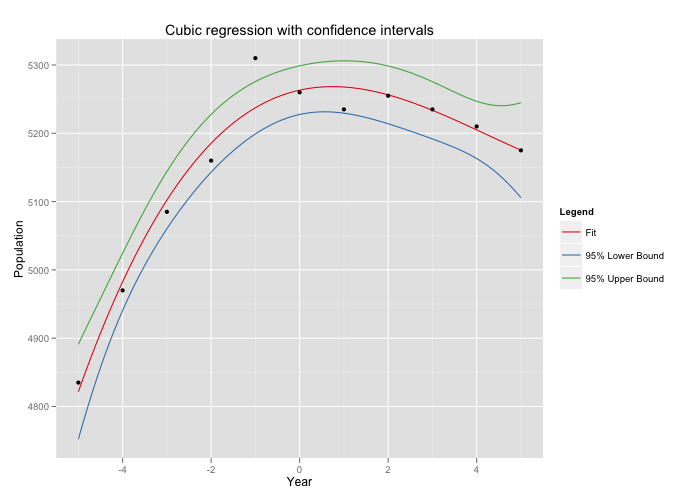
\includegraphics[width=\textwidth]{./RCode/CubicRegression.png}
    \end{figure}

    We can implement this algorithm in R as follows:

\begin{lstlisting}
library("ggplot2")
library("reshape2")

# Raw data
simulation.xs <- c(1959, 1960, 1961, 1962, 1963, 1964, 1965, 1966, 1967, 1968, 1969)
simulation.ys <- c(4835, 4970, 5085, 5160, 5310, 5260, 5235, 5255, 5235, 5210, 5175)
simulation.df <- data.frame(pop = simulation.ys, year = simulation.xs)

# Rescale years
simulation.df$year <- simulation.df$year - 1964

# Generate regression, construct confidence intervals
fit <- lm(pop ~ year + I(year^2) + I(year^3), data=simulation.df)
xs <- seq(-5, 5, 0.1)
fit.confidence <- predict(fit, data.frame(year=xs), interval="confidence", level=0.95)


# Create data frame containing variables of interest
df <- as.data.frame(fit.confidence)
df$year <- xs
df <- melt(df, id.vars="year")

p <- ggplot()
p <- p + geom_line(aes(x=year, y=value, colour=variable),
                   df)
P <- p + geom_point(aes(x=year, y=pop), 
                    simulation.df)
p <- p + scale_x_continuous('Year') 
p <- p + scale_y_continuous('Population')
p <- p + opts(title="Cubic regression with confidence intervals")
p <- p + scale_color_brewer(name="Legend",
        labels=c("Fit", 
                 "95% Lower Bound", 
                 "95% Upper Bound"), 
        palette="Set1")
\end{lstlisting}

    TODO: Part 2.
\end{proof}

\begin{exer}[The Gauss-Markov Theorem]
    \begin{enumerate}
    \item Prove the Gauss-Markov theorem: the least squares estimate of a parameter $a^T\beta$ has a variance no bigger than that of any other linear unbiased estimate of $a^T\beta$.

    \item Secondly, show that if $\hat V$ is the variance-covariance matrix of the least squares estimate of $\beta$ and $\tilde V$ is the variance covariance matrix of any other linear unbiased estimate, then $\hat V \leq \tilde V$, where $B \leq A$ if $A - B$ is positive semidefinite.
    \end{enumerate}
\end{exer}

\begin{proof}
    Let $\hat \theta = a^T \hat \beta = a^T(X^TX)^{-1}X^T y$ be the least squares estimate of $a^T \beta$.  Let $\tilde \theta = c^T y$ be any other unbiased linear estimator of $a^T \beta$.  Now, let $d^T = c^T - a^T(X^{-1}X)^{-1}X^T$.  Then as $c^T y$ is unbiased, we must have \begin{align*}
        E(c^T y) &= E\left( a^T(X^{T}X)^{-1}X^T + d^T\right) y \\
                &= a^T\beta + d^T X\beta \\
                &= a^T\beta
    \end{align*} as $c^T y$ is unbiased, which implies that $d^T X = 0$.

    Now we calculate the variance of our estimator.  We have \begin{align*}
        \text{Var}(c^T y) &= c^T \text{Var}(y) c \\
                    &= \sigma^2 c^T c \\
                    &= \sigma^2 \left( a^T(X^{T}X)^{-1}X^T + d^T \right) \left( a^T (X^T X)^{-1} X^T + d^T \right)^T \\
                    &= \sigma^2 \left( a^T (X^T X)^{-1}X^T + d^T\right) \left(X (X^{T}X)^{-1}a + d\right) \\
                    &= \sigma^2 \left( a^T (X^TX)^{-1}X^T X(X^T X)^{-1} a + a^T (X^T X)^{-1} \underbrace{X^T d}_{=0} + \underbrace{d^T X}_{=0}(X^T X)^{-1} a + d^T d \right) \\
                    &= \sigma^2 \left(\underbrace{a^T (X^T X)^{-1} a}_{\text{Var}(\hat \theta)} + \underbrace{d^t d}_{\geq 0} \right)
    \end{align*}

    Thus $\text{Var}(\hat \theta) \leq \text{Var}(\tilde \theta)$ for all other unbiased linear estimators $\tilde \theta$.

    The proof of the matrix version is almost identical, except we replace our vector $d$ with a matrix $D$.  It is then possible to show that $\tilde V = \hat V + D^T D$, and as $D^T D$ is a positive semidefinite matrix for any $D$, we have $\hat V \leq \tilde V$. 
\end{proof}

\begin{exer}
    Show how the vector of least square coefficients can be obtained from a single pass of the Gram-Schmidt procedure.  Represent your solution in terms of the QR decomposition of $X$.  
\end{exer}

\begin{proof}
    Recall that by a single pass of the Gram-Schmidt procedure, we can write our matrix $X$ as \[
        X = Z \Gamma,
        \] where $Z$ contains the orthogonal columns $z_j$, and $\Gamma$ is an upper-diagonal matrix with ones on the diagonal, and $\gamma_{ij} = \frac{\langle z_i, x_j \rangle}{\| z_i \|^2}$. This is a reflection of the fact that by definition, \[
            x_j = z_j + \sum_{k=0}^{j-1} \gamma_{kj} z_k.
            \]

            Now, by the $QR$ decomposition, we can write $X = QR$, where $Q$ is an orthogonal matrix and $R$ is an upper triangular matrix.  We have $Q = Z D^{-1}$ and $R = D\Gamma$, where $D$ is a diagonal matrix  with $D_{jj} = \| z_j \|$.  

    Now, by definition of $\hat \beta$, we have \[
        (X^T X) \hat \beta = X^T y.
        \]  Now, using the $QR$ decomposition, we have \begin{align*}
            (R^T Q^T) (QR) \hat \beta &= R^T Q^T y \\
            R \hat \beta &= Q^T y
        \end{align*}
    As $R$ is upper triangular, we can write \begin{align*}
        R_{pp} \hat \beta_p &= \langle q_p, y \rangle \\
        \| z_p \| \hat \beta_p &= \| z_p \|^{-1} \langle z_p, y \rangle \\
        \hat \beta_p &= \frac{\langle z_p, y \rangle}{\| z_p \|^2}
    \end{align*} in accordance with our previous results.  Now, by back substitution, we can obtain the sequence of regression coefficients $\hat \beta_j$.  As an example, to calculate $\hat \beta_{p-1}$, we have \begin{align*}
        R_{p-1, p-1} \hat \beta_{p-1} + R_{p-1,p} \hat \beta_p &= \langle q_{p-1}, y \rangle \\
        \| z_{p-1} \| \hat \beta_{p-1} + \| z_{p-1} \| \gamma_{p-1,p} \hat \beta_p &= \| z_{p-1} \|^{-1} \langle z_{p-1}, y \rangle 
    \end{align*} and then solving for $\hat \beta_{p-1}$. This process can be repeated for all $\beta_j$, thus obtaining the regression coefficients in one pass of the Gram-Schmidt procedure.
\end{proof}

\begin{exer}
    Consider the ridge regression problem (3.41).  Show that this problem is equivalent to the problem \[
        \hat \beta^c = \argmin_{\beta^c} \left( \sum_{i=1}^{N} \left( y_i - \beta^c_0 - \sum_{j=1}^{p}(x_{ij} - \hat x_j) \beta^c_j \right)^2 + \lambda \sum_{j=1}^{p}{\beta_j^c}^2 \right)^2.
        \]
\end{exer}

\begin{proof}
    Consider rewriting our objective function above as  \[
        L(\beta^c) = \sum_{i=1}^{N}\left(y_i - \left(\beta_0^c - \sum_{j=1}^{p} \bar x_j \beta_j^c \right) - \sum_{j=1}^p x_{ij} \beta_j^c \right)^2 + \lambda \sum_{j=1}^p {\beta_j^2}^2
        \]
    Note that making the substitutions \begin{align*}
        \beta_0 &\mapsto \beta_0^c - \sum_{j=1}^p \hat x_j \beta_j \\
        \beta_j &\mapsto \beta^c_j, j = 1, 2, \dots, p
    \end{align*} that $\hat \beta$ is a minimiser of the original ridge regression equation if $\hat \beta^c$ is a minimiser of our modified ridge regression.  

    The modified solution merely has a shifted intercept term, and all other coefficients remain the same.  
\end{proof}

\begin{exer}
    Show that the ridge regression estimate is the mean (and mode) of the posterior distribution, under a Gaussian prior $\beta \sim N(0, \tau \mathbf{I})$, and Gaussian sampling model $y \sim N(X \beta, \sigma^2 \mathbf{I})$.  Find the relationship between the regularization parameter $\lambda$ in the ridge formula, and the variances $\tau$ and $\sigma^2$.
\end{exer}

\begin{exer}
    Assume 
    \[ y_i \sim N(\beta_0 + x_i^T \beta, \sigma^2), i = 1, 2, \dots, N \] and the parameters $\beta_j$ are are each distributed as $N(0, \tau^2)$, independently of one another.  Assume $\sigma^2$ and $\tau^2$ are known, show that the minus log-posterior density of $\beta$ is proportional to 
    \[ \sum_{i=1}^N \left( y_i - \beta_0 - \sum_{j=1}^p x_{ij} \beta_j \right)^2 + \lambda \sum_{j=1}^p \beta_j^2 \]
    where $\lambda = \frac{\sigma^2}{\tau^2}$.  
\end{exer}

\begin{exer}
    Consider the $QR$ decomposition of the uncentred $N \times (p+1)$ matrix $X$, whose first column is all ones, and the SVD of the $N \times p$ centred matrix $\tilde X$.  Show that $Q_2$ and $U$ share the same subspace, where $Q_2$ is the submatrix of $Q$ with the first column removed.  Under what circumstances will they be the same, up to sign flips?
\end{exer}

\begin{proof}
    Denote the columns of $X$ by $x_0, \dots, x_{p}$, the columns of $Q$ by $z_0, \dots, z_p$, the columns of $\tilde X$ by $\tilde x_1, \dots, x_n$, and the columns of $U$ by $u_1, \dots, u_p$.  Without loss of generality, we can assume that for all $i$, $\| x_i \| = 1$ and that $X$ is non-singular (this cleans up the proof somewhat).


    First, note that by the QR decomposition, we have that $\text{span}(x_0, \dots, x_j) = \text{span}(z_0, \dots, z_j)$ for any $0 \leq j \leq p$.  

    By our assumption, we have that $\tilde x_i = x_i - \bar x_i \mathbf{1}$ for $i = 1, \dots, p$.  Thus we can write $\tilde x_i = \sum_{j \leq i} \alpha_j z_j$, and as the $z_j$ are orthogonal, we must be able to write $\tilde x_i$ in terms of $z_j$ for $j = 1, 2, \dots, i$.  Thus $\text{span}(\tilde x_1, \dots, \tilde x_i) = \text{span}(z_1, \dots, z_i)$.  

    Finally, we calculate $\text{span}(u_1, \dots, u_p)$.  We have that $U$ is a unitary $N \times p$ matrix, and thus the columns of $U$ span the column space of $\tilde X$, and thus the span of $Q_2$ is equal to the span of $U$.  

    TODO: When is $Q_2$ equal to $U$ up to parity?  Is it where columns of 
\end{proof}
\begin{exer}[Forward stepwise regression]
    Suppose that we have the $QR$ decomposition for the $N \times q$ matrix $X_1$ in a multiple regression problem with response $y$, and we have an additional $p - q$ predictors in matrix $X_2$.  Denote the current residual by $r$.  We wish to establish which one of these additional variables will reduce the residual-sum-of-squares the most when included with those in $X_1$.  Describe an efficient procedure for doing this.
\end{exer}

\begin{proof}
    Select the vector $x_{j'}$ where
    \begin{align*}
        x_{j'} = \argmin_{j = q+1, \dots, p} \left| \left\langle \frac{x_q}{\| x_q \|}, r \right\rangle \right| 
    \end{align*}
    
    This selects the vector that explains the maximal amount of variance in $r$ given $X_1$, and thus reduces the residual sum of squares the most.  It is then possible to repeat this procedure by updating $X_2$ as in Algorithm 3.1.
\end{proof}
\begin{exer}[Backward stepwise regression]
    Suppose that we have the multiple regression fit of $y$ on $X$, along with standard errors and $z$-scores.  We wish to establish which variable, when dropped, will increase the RSS the least.  How would you do this?
\end{exer}

\begin{proof}
    By Exercise 3.1, we can show that the F-statistic for dropping a single coefficient from a model is equal to the square of the corresponding $z$-score.  Thus, we drop the variable that has the lowest squared $z$-score from the model.
\end{proof}

\begin{exer}
    Show that the solution to the multivariate linear regression problem (3.40) is given by (3.39).  What happens if the covariance matrices $\Sigma_i$ are different for each observation?
\end{exer}

\begin{exer}
    Show that the ridge regression estimates can be obtained by OLS on an augmented data set.  We augment the centred matrix $X$ with $p$ additional rows $\sqrt{\lambda} \mathbf{I}$, and augment $y$ with $p$ zeroes. 

\end{exer}
\begin{proof}
    For our augmented matrix $X_1$, equal to appending $\sqrt{\lambda I}$ to the original observation matrix $X$, we have that the $RSS$ expression for OLS regression becomes \begin{align*}
        RSS &= \sum_{i=1}^{N+p} \left(y_i - \sum_{j=1}^p x_{ij} \beta_j \right)^2 \\
            &= \sum_{i=1}^{N} \left( y_i - \sum_{j=1}^p x_{ij} \beta_j \right)^2 + \sum_{i = N + 1}^{N+p} \left(\sum_{j=1}^p x_{ij} \beta_j \right)^2 \\
            &= \sum_{i=1}^{N} \left( y_i - \sum_{j=1}^p x_{ij} \beta_j \right)^2 + \sum_{j=1}^p \lambda \beta_j^2 
    \end{align*} which is the objective function for the ridge regression estimate.
\end{proof}
